%!TEX root = ../Arduino.tex
%Kapitel 3%
\section{RGB-LEDs}
RGB-LED bestehen aus 3 farbigen (rot, grün und blau) LEDs. Die eine gemeinsame Kathode (Minuspol) besitzen. Sie eignen sich dazu Mischfarben, die aus den drei Grundfarben aufgebaut sind darzustellen. Mit zwei Potentiometer und einem weißen Tischtennisball können schöne Farbeffekte erzeugt werden.      

\marginfigure{Kapitel3/Bilder/rgb-led}{RGB-LED}{fig:rgb-led}

\subsection{Farben mit Potentiometer mischen}

An vielen elektronischen Geräten findet man Regler, an denen man drehen oder schieben kann. Dahinter stecken meistens Potentiometer, kurz „Poti“ genannt. Sie sind regelbare Widerstände und haben meistens drei Anschlüsse. Üblicherweise ist der linke Anschluss an einem Ende einer Kohleschicht befestigt, der rechte Anschluss am anderen Ende. Der mittlere Anschluss, genannt Mittelabgriff, ist mit einem Kontakt verbunden, der auf der Kohleschicht schleift und beim Drehen oder Schieben verschoben wird. Da die Kohlebahn relativ schlecht leitet, fließt ein Strom leichter durch ein kurzes dünnes Stück Kohlespur als durch ein langes ebenso dünnes Stück Kohle. Beim Drehen des Potentiometers wird also der elektrische Widerstand zwischen dem Mittelabgriff und jedem der anderen Anschlüsse verändert. Wenn man Potentiometer kauft, ist meistens der Maximalwiderstand angegeben. Der minimale Widerstand beträgt nahezu $0\Ohm$.

\subsection{Aufbau der Schaltung}
RGB-LEDs sind empfindlich und relativ teuer, das heißt sie dürfen nur mit Vorwiderstand betrieben werden. Wenn du die Schaltung ohne die $220\Ohm$-Widerstände aufbaust bist du schnell um ca. 1 Euro ärmer, aber um eine Kaputte RGB-LED reicher! Ansonsten erfolgt der Aufbau genau wie mit normalen LEDs. Der längste Anschluss ist die gemeinsame Kathode (Minus-Pol) und wird mit GND verbunden. Die anderen Pins werden mit PWM-Ports verbunden.   
\margininfo{Es gibt auch Anoden RGB-LEDs, der gemeinsamme Pin ist dann die Anode (plus Pol).}

\subsection{Aufgaben}

\subsubsection{Aufgabe 1}
Baue zuerst die Schaltung entsprechend Abb. \ref{fig:rgb-led} auf. Öffne den Beispiel-Sketch Beispiele/01Basic/Fade und ändere den Sketch so ab, dass die rote LED über den digitalen PIN 11, die blaue auf dem digitalen PIN 12 und die grüne LED auf dem digitalen PIN 13 angesteuert werden können. 

Ändere für die verschieden Ports den brightness-Wert und versuche so verschiedene Farben zu erzeugen. 

\subsubsection{Aufgabe 2}
Für dieses Aufgabe benötigst du ein größeres Bread-Board. Bau dann die Schaltung entsprechend der Abb. \ref{fig:rgb-mischer} auf. Lade anschließend den Beispiel-Sketch Beispiele/10StarterKit/p04\_ColorMixingLamp. Anstelle der Photo-Widerstände werden bei dieser Aufgabe die Potis verwendet. Mache dich mit der Funktionsweise dieses Sketches vertraut.  

\marginfigure{Kapitel3/Bilder/rgb-mischer}{RGB Mischer}{fig:rgb-mischer} 

\subsubsection{Aufgabe 3 Projekt}
Wenn du die Aufgabe 1 und 2 gut verstanden hast, dann solltest du jetzt in der Lage sein RGB-LED in verschiedenen Projekten zu verwenden. Vielleicht wäre es eine gute Übung für dich dein optisches Thermometer anstatt mit 3 LEDs (rot, gelb und grün) mit einer RGB-LED neu aufzubauen. Eine weitere Idee wäre es eine optische Abstandswarnung zu bauen. Im Abschnitt \ref{sec:farbenraum} ist noch Hintergrundwissen zur Farberzeugung mit Hilfe einer RGB-LED zu finden.     

\subsection{Der Farbenraum}\label{sec:farbenraum}
Ein RGB-Farbraum ist ein additiver Farbraum, der Farbwahrnehmungen durch das additive Mischen dreier Grundfarben (Rot, Grün und Blau) nachbildet. Das Farbsehen des Menschen ist von drei Zapfentypen geprägt. 

Dieser Farbraum wird für selbstleuchtende (farbdarstellende) Systeme benutzt, die dem Prinzip der Additiven Farbmischung unterliegen, daher auch als Lichtmischung bezeichnet. Nach Graßmanns Gesetzen lassen sich Farben durch drei Angaben definieren, im RGB-Farbraum sind dies der Rot-, der Grün- und der Blauanteil. Die konkrete Form des Farbraums hängt vom jeweils konkreten technischen System ab, für das der jeweilige Farbraum bestimmt wurde.


\marginfigure{Kapitel3/Bilder/rgb-color-space}{RGB Farbenraum}{fig:rgb-color-space}



\sectionInformatik{C Sprachelemente: millis() versus delay()}
\label{sec:millis}
Bisher hast du eine LED mit Hilfe der delay()-Funktion ein und ausgeschaltet. Das ist in Ordnung,  solange das Arduino Board nur eine Aufgabe hat. Aber wie sollte mit dem delay()-Befehl folgende Aufgabe löst werden?

\subsubsection{Aufgabe 1}

Baue die Schaltung aus Abbildung \ref{fig:delay-millis} auf. Die rote LED soll blinken (eine Sekunde an, eine Sekunde aus). Die grüne LED leuchten, wenn der Push-Buttom gedrückt ist und nicht leuchten wenn der Push-Buttom losgelassen wird.

\marginfigure{Kapitel3/Bilder/delay_mills.png}{}{fig:delay-millis}

\subsubsection{Lösungs Hinweis}
Um diese Aufgabe zu lösen, muss man das an- und ausschalten der roten LED so steuern, dass der Arduino nicht blockiert wird. Ein mögliche Lösung bietet der millis()-Befehl. Wenn millis() aufgerufen wird, dann gibt er die Zeit in Millisekunden zurück, seit der Arduino das aktuelle Programm ausführt. 

\begin{multicols}{2}
\begin{arduinoCode}{Aufbau einer C-Funktion}{lst:millis}
const int blinkLed = 13;
long time = 0;  (*@ \tikzmark{time} @*)
boolean stateLed = false; (*@\tikzmark{stateLed} @*)

void setup() {                
  pinMode(blinkLed, OUTPUT);
  time = millis();  
}

void loop() {
  if (millis()-time > 1000){ 
    stateLed = !stateLed; (*@\tikzmark{statechange} @*)
    time = millis();
    digitalWrite(blinkLed, stateLed); (*@\tikzmark{statewrite} @*)
  } 
}
\end{arduinoCode}
\columnbreak
\vfill\null 
\begin{itemize}
  \itemsep20pt
    \item[] \tikzmarkcomment{item1}{Aktuelle Ausführzeit des Sketches wird gespichert}
    \item[] \tikzmarkcomment{item2}{Aktueller Zustand der blickLed wird gespeichert}
    \item[] \tikzmarkcomment{item3}{Zustand der blickLed wird nach einer Sekunde geändert}
    \item[] \tikzmarkcomment{item4}{Zustand der blickLed wird übertragen}
 \end{itemize}
\vfill \null

\begin{tikzpicture}[remember picture,overlay]
  \path[red, thick,-] (time.east) edge [out=0 , in=180] (item1);
  \path[red, thick,-] (stateLed.east) edge [out=0 , in=180] (item2);
  \path[red, thick,-] (statechange.east) edge [out=0 , in=180] (item3);
  \path[red, thick,-] (statewrite.east) edge [out=0 , in=180] (item4);
\end{tikzpicture}
\end{multicols}
\margininfo{! ist der Negations-Operator}
Mit Hilfe des Listings \ref{lst:millis} sollte es dir möglich sein Aufgabe 1 zu lösen.

%\subsection{Call Backs}



%%%%%%%%%%%%%%%%%%%%%%%%%%%%%%%%%%%%%%%
%% Lautsprecher %%%%%%%%%%%%%%%%%%%%%%%
%%%%%%%%%%%%%%%%%%%%%%%%%%%%%%%%%%%%%%%
\section{Lautsprecher}

In Kapitel \ref{chapter:1} haben wir zur Visualisierung des digitalen Ausgänge LED`s benutzt.
Statt optischer Ausgaben über LEDs können aber auch akustische Ausgaben erzeugt werden. 
Dazu wird ein Lautsprecher an einen Ausgang des Mikrokontrollers angehängt und schnell ein und 
ausgeschaltet. Dies erzeugt Kräfte in der Spule des Lautsprechers. Diese Kräfte lassen die Membran
im Lautsprecher hin und her schwingen und wir hören die entsprechende Frequenz der 
Membranschwingung als Ton.

\subsection{Lautstärkeregelung mit einem Potentiometer}

Ihr sollt hier ein Potentiometer verwenden, um die Lautstärke des ohnehin recht leisen Tons noch leiser einstellen, bis der Ton schließlich unhörbar leise wird. Dazu muss die Stromstärke im Lautsprecher verringert werden - der zusätzliche veränderbare Widerstand muss also zwischen den Port und den Lautsprecher oder - das ist genau so gut - zwischen den Lautsprecher und den $5\V$ des digitalen Ports geschaltet werden. 

\marginfigure{Kapitel3/Bilder/ton}{Arduino mit Piezolautsprecher}{fig:ton}

\subsection{Aufgaben}

Baue die Schaltung mit dem Lautsprechen entsprechend Abb. \ref{fig:ton} auf. 

\subsubsection{Aufgabe 1}
Für deine ersten Töne genügt es den „Blink“ Sketch entsprechend anpassen. Dazu muss du den Befehl Delay (Millisekunden) durch ein DelayMicroseconds (Microsekunden) ersetzen und auf den Arduino laden. Wenn dein Lautsprechen mit dem richtigen Port verbunden ist solltest du einen konstanten Ton hören.



\subsubsection{Aufgabe 2}
Für die folgende Aufgabe solltest du auf deine Mitschüler Rücksicht nehmen, indem du ein Potentiometer zur Lautstärke-Regelung einbaust. Bau dazu deine Schaltung entsprechend der Abb. \ref{fig:ton-poti} um. 
\marginfigure{Kapitel3/Bilder/ton-poti}{Lautsprecher mit Poti}{fig:ton-poti}   
In der Tabelle \ref{tab:Tonleiter} sind die Frequenzen der Töne einer C-Dur Tonleiter aufgeführt.
\begin{table}[h]

\begin{center}

\tikzset{ 
    table/.style={
        matrix of nodes,
        row sep=-\pgflinewidth,
        column sep=-\pgflinewidth,
        nodes={
            rectangle,
            draw=black,
            align=center
        },
        minimum height=1.5em,
        text depth=0.5ex,
        text height=2ex,
        nodes in empty cells,
%%
        every even row/.style={
            nodes={fill=gray!20}
        },
        column 1/.style={
            nodes={text width=0.3\textwidth}
        },
        row 1/.style={
            nodes={
                fill=black!80,
                text=white,
                font=\bfseries
            }
        }
    }
}

\begin{tikzpicture}
\matrix (first) [table,text width=6em]
{   
  Ton & c & d  & f & g & a \\
  Frequenz ($\Hz$)& 294 & 329 & 349 & 392 & 440 \\
};
 \end{tikzpicture}
\end{center}
\caption{C-Dur Tonleiter mit Frequenzen }
\label{tab:Tonleiter}
\end{table}%
\begin{itemize}
  \item[a)] Berechnen anhand der Werte aus der Tabelle die Perionendauer für die verschiedenen Töne. Um einen Ton jetzt zu erzeugen, muss der digitale Pin jeweils für die Hälfte der Periodendauer 'HIGH' bwz. 'LOW' sein. 
  \item[b)] Schreibe einen Sketch, der das Lied Alle meine Endchen spielt. 
  \item[c)] Schreibe eine C Funktion: \\
  void playTone(int tone, int duration) \\
  Die einen gegebenen Ton 'tone' für eine bestimmte Zeit 'duration' abspielt. Schreibe den Sketch aus Teil b) entsprechend um, dass jetzt diese Funktion verwendet wird. 
\end{itemize}

\subsubsection{Aufgabe 3 Projekt}
 Der Beispiel-Sketch „Examples/Digital/Melody“ macht das ganze etwas eleganter. Lade den Sketch auf dein Board. Wenn das Abspielen klappt, kannst du versuchen die Melodie zu ändern. Dazu muss du allerdings verstanden haben, wie das Beispiel genau funktioniert. 

Wichtig: Du kannst nur die Töne verwenden, die in der Datei pitches.h definiert sind.

\subsection{Zum weiterlese:}
\begin{itemize}
\item \url{http://arduino.cc/en/Tutorial/Tone}
\end{itemize}

\section{Der Transistor als Schalter oder zur  Verstärkung}
\marginfigure{Kapitel3/Bilder/ndet}{Nachbau des ersten Transistors (CC Attribution-Share Alike 3.0 Unported by \href{https://upload.wikimedia.org/wikipedia/commons/6/62/Nachbau_des_ersten_Transistors.jpg}{commons.wikimedia.org})}{}
Ein Transistor ist ein elektronisches Bauelement zum Schalten und Verstärken von elektrischen Signalen, ohne dabei mechanische Bewegungen auszuführen. Transistoren sind die weitaus wichtigsten „aktiven“ Bestandteile elektronischer Schaltungen, welche beispielsweise in der Nachrichtentechnik, der Leistungselektronik und in Computersystemen eingesetzt werden. Besondere Bedeutung haben Transistoren in integrierten Schaltkreisen, was die derzeit weit verbreitete Mikroelektronik ermöglicht.

Es gibt zwei wichtige Gruppen von Transistoren, nämlich Bipolartransistoren und Feldeffekttransistoren (FET).

Der Metall-Oxid-Halbleiter-Feldeffekttransistor (englisch metal-oxide-semiconductor field-effect transistor, MOSFET auch MOS-FET, selten MOST) gehört zu den Feldeffekttransistoren mit isoliertem Gate. Er ist den Metall-Isolator-Halbleiter-Feldeffekttransistoren (MISFET) zuzurechnen. Obwohl heute dotiertes Polysilizium als Gate-Material vorherrscht, wurde die Bezeichnung MOSFET beibehalten. 

\begin{figure}[h]
  \begin{center}
  \subfigure[PinOut: MOSFET und bipolarer Transistor]{\includegraphics[width=0.3\textwidth]{Kapitel3/Bilder/transistor_pinout}}\qquad\qquad
  \subfigure[Schaltzeichen: MOSFET und bipolarer Transistor]{\begin{circuitikz} %
  \draw (1,3) node[nigfete ](nigfete) {} 
  (nigfete.G)node[anchor=east] {G}
  (nigfete.S)node[anchor=north] {S}
  (nigfete.D)node[anchor=south] {D};
  \draw ($(nigfete)-(0.18,0)$) circle [radius=18pt];
  \draw (4,3) node[npn] (npn) {}
  (npn.base)node[anchor=east] {B}
  (npn.collector)node[anchor=south] {C}
  (npn.emitter)node[anchor=north] {E};
  \draw ($(npn)-(0.18,0)$) circle [radius=18pt]; 
  \draw (0,0) circle; 
  \end{circuitikz}}
  \label{fig:pinout}
  \caption{MOSFET (n-Kanal) und bipolaren Transistor (npn)}
  \end{center}
\end{figure}


\subsection{Einsatzmöglichkeiten für einen bipolaren Transistor}
Grundsätzlich gibt es  zwei verschiedene Möglichkeiten einen bipolaren Transistor zu betreiben:
\begin{itemize}
\item Proportionalbetrieb: Der Kollektor- bzw. Emitterstrom ist proportional zum Basisstrom. Je größer der Basisstrom desto größer der Kollektorstrom. Den Verstärkungsfaktor selbst kannst du im Datenblatt nachlesen. Da die Spannung $U_{CE}$ recht groß ist erwärmt sich der Transistor (Verlustleistung!).
\item Schaltbetrieb: Der Transistor leitet entweder voll oder sperrt komplett. Der Basistrom muss groß genug sein, um den Kollektor- bzw. Emitterstrom nicht zu begrenzen. Ein Basiswiderstand ist für den Schutz des digitalen Ports nötig, nicht für den Betrieb des Transistors. Ohne Basiswiderstand würde der Ausgang des Arduino fast kurzgeschlossen, denn die Vorwärtsspannung U$_{BE}$ ist in der Regel etwa 0,7 V (Achtung: für jeden Transistor muss dieser Wert aus dem Datenblatt entnommen werden). Du benötigst deshalb einen Vorwiderstand von etwa 100$\Ohm$, der den Strom durch den digitalen Port auf maximal $40\mA$ begrenzt.
\end{itemize}

Um die Musik in vernünftiger Lautstärke über einen Lautsprecher auszugeben reicht die maximale zulässige Stromstärke der digitalenPots nicht aus.

\margininfo{Möchte man einen Transistor nur als Schalter verwenden, so ist ein MOSFET einem bipolarem Transistor vorzuziehen, da ein MOSFET praktisch keine Verlustleistung hat.}
\subsection{Aufbau der Schaltung}

Beachte, dass du je nach Transistor im Datenblatt nachsehen musst, wo sich die Basis, der Collector und der Emitter befinden.

\begin{figure}[h]
\begin{center}
\begin{circuitikz}
  \draw (-2,0) node[anchor=east]{GND}
  (4,0) to[short, -o] (-2,0)
  (1,1) node[npn](s2) {} 
  (s2.base) to[R,l=$R_{B}$, -o] ($(s2.base)-(2,0)$)
  ($(s2.base)-(2,0)$) node[anchor=east] {Pin}
  (1,0) to[short, *-]  (s2.south east)
  (1,2) to[short]  (s2.north east)
  (1,2) to[R, l=$R_{Last}$] (1,4)
  (1,4) to[short] (4,4)
  (4,0) to[battery, l=$9V$] (4,4);
  \draw ($(s2)-(0.18,0)$) circle [radius=18pt];\end{circuitikz}
  \caption{Grundschaltung bipolarer Transistor (npn)}
  \label{fig:brueckenschaltung}
\end{center}
\end{figure}

\subsection{Aufgaben}
Baue die Schaltung nach Abb. \ref{fig:ton-npn}. Beachte, dass du für den verwendeten Transistor im Datenblatt nachsehen musst, wo sich die Basis, der Collector und der Emitter befinden.
\marginfigure{Kapitel3/Bilder/ton-npn}{npn-Transistor}{fig:ton-npn}

\subsubsection{Aufgabe 1}
Wenn du dich überzeugt hast, dass die Schaltung richtig aufgebaut ist. Kannst du die Wirkung des bipolaren Transistor und des Potis mit Hilfe deines Melodie-Sketch testen.

\clearpage
\subsection{MOSFET als Schalter}

Auch mit einem MOSFET ist es möglich den Lautsprecher lauter zu bekommen. MOSFET werden dann bevorzugt eingesetzt, wenn die Verlustleistung entscheidend wird.
Da es keine Collector-Source-Strom gibt, ist die Verlustleistung Praktisch Null. Der zweite Einsatz ist wenn sehr große Lasten geschalter werden, so steuert man ein Relais üblicherweise mit einem MOSFET an.

\margininfo{Natürlich kann eine MOSFET auch als Verstärker geschaltet werden. Da es bei ihm keinen Gate-Source-Strom gibt, wird mit Hilfe der Gate-Source-Spannung der Collector-Source-Strom geschaltet. Da aber ohne Spannungsteiler immer $0V$ oder $5V$ Potentialunterschied anliegen, schaltet der MOSFET eben nur.}

\subsection{Aufbau der Schaltung}

\begin{figure}[h]
\begin{center}
\subfigure[Direkte Methode: N-Kanal MOSFET (NFET)\label{fig:nfet}]{ 
 \begin{circuitikz} \draw
(0,0) node[anchor=east]{GND}
  (3,0) to[short, -o] (0,0)
  (1,1) node[nigfete ](s2) {} 
  (s2.G) to[short, o-] (s2.G)
  (s2.G) node[anchor=east] {Pin}
  (1,0) to[short, *-]  (s2.south east)
  (1,2) to[short]  (s2.north east)
  (1,2) to[R, l=$R_{Last}$] (1,4)
  (1,4) to[short] (3,4)
  (3,0) to[battery, l=$9V$] (3,4);
  \draw ($(s2)-(0.18,0)$) circle [radius=18pt];\end{circuitikz}}\qquad 
\subfigure[Direkte Methode: P-Kanal MOSFETs (PFET)\label{fig:pfet}]{ 
 \begin{circuitikz} 
  \draw
  (0,0) node[anchor=east]{GND}
  (3,0) to[short, -o] (0,0)
  (1,1) node[pigfete ](s2) {} 
  (s2.G) to[short, o-] (s2.G)
  (s2.G) node[anchor=east] {Pin}
  (1,0) to[short, *-]  (s2.south east)
  (1,2) to[short]  (s2.north east)
  (1,2) to[R, l=$R_{Last}$] (1,4)
  (1,4) to[short] (3,4)
  (3,0) to[battery, l=$9V$] (3,4);
  \draw ($(s2)-(0.18,0)$) circle [radius=18pt];\end{circuitikz}}
  \caption{Grundschaltung MOSFET}
  \label{fig:brueckenschaltung}
\end{center}
\end{figure}


Zu beachten ist, dass zwischen Gate und Source und zwischen Gate und Drain eine Kapazität existiert, welche bei jedem Umschalt-Vorgang umgeladen werden muss. Besonders bei höheren Frequenzen (größer $ 10\kHz$) ist zur Strombegrenzung zwischen Gate und dem digitalen Port des Arduinos ein Widerstand sinnvoll. Übliche Werte dafür sind $50 - 100\Ohm$. 

\subsection{Aufgaben}
Baue die Schaltung mit dem Lautsprecher und n-MOSFET Transistor entsprechend Abb. \ref{fig:ton-nfet} auf.
\marginfigure{Kapitel3/Bilder/ton-nfet.png}{n-MOSFET Verstärker}{fig:ton-nfet} Anstatt der Batterie wird hier die $5\V$ des Arduino Uno verwendet.   
 
\subsubsection{Aufgabe 1}
Wenn du dich überzeugt hast, dass die Schaltung richtig aufgebaut ist. Kannst du die Wirkung des MOSFETs mit Hilfe deines Melodie-Sketch testen.

\clearpage
\section{Peltier-Element}

Das Peltier- oder thermoelektrische Element, ist  ein Bauteil, das Wärme (Entropie) von einer Seite auf eine andere übertragen kann, wenn ein Strom angelegt wird. Es kann zum heizen oder  kühlen verwenden werden, dazu muss die Stromrichtung umgepolt werden. Das Peltier-Element kann mit zu einer Spannung von $15,4\V$ und einem maximalen Strom von $7A$ versorgt werden.


\subsection{Ausbau der Schaltung}

Du benötigst ein Peltier-Element, einen N-Mosfet,
einen $1000\Ohm$ Widerstand und einen Batteriehalter mit zwei Akkus. Die Abb. \ref{fig:peltier} zeigt den Aufbau der Schaltung.   
\marginfigure{Kapitel3/Bilder/peltier}{Peltier-Element}{fig:peltier}

\subsection{Der Beispiel-Sketch}


\begin{multicols}{2}
\begin{arduinoCode}{Peltier Kühlung}{lst:peltier}
int peltierPin = 3; 
int power = 0; 
int peltLevel = 0; (*@ \tikzmark{init} @*) 

void setup(){
  Serial.begin(9600);
  pinMode(peltierPin, OUTPUT);
}

void loop(){
  if(Serial.available() > 0) {
    int deltaPower = Serial.read();
    power += deltaPower
    peltLevel = map(power, 0, 99, 0, 255);
  }
  Serial.print("Power= ");
  Serial.print(power);
  analogWrite(peltierPin, peltLevel); (*@ \tikzmark{write} @*)
}
\end{arduinoCode}
\columnbreak
\vfill\null 
\begin{itemize}
  \itemsep20pt
    \item[] \tikzmarkcomment{item1}{This is a value from 0 to 255 that actually controls the MOSFET}
    \item[] \tikzmarkcomment{item2}{Write this new value out to the port
}
 \end{itemize}
\vfill \null

\begin{tikzpicture}[remember picture,overlay]
  \path[red, thick,-] (init.east) edge [out=0 , in=180] (item1);
  \path[red, thick,-] (write.east) edge [out=0 , in=180] (item2);
\end{tikzpicture}
\end{multicols}



Das besondere am Sketch aus Listing \ref{lst:peltier} ist, dass das Verhalten des Arduinos über die serielle Schnittstelle gesteuert wird. Man sollte die Schaltung nicht zu lange betreiben, das durch den MOSFET schon einiges an Energie fließt und sich dieser durch die Verlustleistung stark aufheizen kann.


\subsection{Aufgaben}

Bau die Schaltung entsprechend Abb. \ref{fig:peltier} auf. Achte darauf, dass der N-Mosfet richtig eingebaut ist. 
\margininfo{Achtung: Der Mosfet kann bei lagen Betrieb heiß werden!} 

\subsubsection{Aufgabe 1}

Lade den Beispiel-Sketch \ref{lst:peltier} auf deinen Arduino und öffne anschließend das serielle Terminal. Mache dich mit der Funktionsweise des Sketch vertraut und dokumentier alle noch nicht dokumentierten Befehle.

\subsubsection{Aufgabe 2}
Erweitere deine Schaltung und deinen Sketch um einen Temperatur-Sensoren. Messe die Temperatur auf beiden Seiten des Peltier-Elements und gibt die gemessene Temperatur ebenfalls über die serielle Schnittstelle aus.
  
\subsubsection{Aufgabe 3 Projekt}
Erweitere deine Schaltung um ein zweites Peltier-Element das das Heizung geschaltet ist. Erweitere deinen Sketch, so dass eine vorgegebenen Temperatur in einem abgeschlossenen Behälter gehalten werden kann.    


\section{Servomotor}
Soll ein Arduino etwas bewegen, dann gibt es mehrere Möglichkeiten dies zu tun. Es können normale 
Elektromotoren, Schrittmotoren oder Modellbauservos benutzt werden. Modellbauservos haben den 
Vorteil, dass sie leicht anzusteuern sind, und die notwendige Leistungselektronik bereits im Servo 
eingebaut ist. Auch benötigt man keine aufwändigen Rückmeldungen von der Mechanik um eine 
bestimmte Position anzufahren oder um die Schrittverluste eines Schrittmotors auszugleichen. 
Ein Servo findet ganz von alleine nach dem Einschalten seine Neutralposition. 

Servos gibt es in allen möglichen Preiskategorien, wobei die Unterschiede in dem Drehmoment des Motors bzw. in der Qualität des integrierten Getriebes liegen. 

Ein Servo besteht aus mehreren logischen Komponenten

\begin{itemize}
\item Elektronik für die Pulsauswertung
\item Elektronik für eine Regelschleife
\item Leistungselektronik zur Ansteuerung eines Motors
\item der Motor samt Getriebe
\item Positionsauswertung
\end{itemize}
Aus diesen Komponenten wird eine Regelschleife gebildet, so dass der Motor einem 
Positionssignal nachgeführt wird. Am Motor ist ein Getriebe angeflanscht, welches wiederum 
die Abtriebsscheibe bewegt, an der die Bewegung mechanisch abgegriffen werden kann.

\begin{figure}[h]

\centering
\begin{tikzpicture}
[node distance = 1cm, auto,font=\footnotesize,
% STYLES
every node/.style={node distance=3cm, rounded corners},
% The comment style is used to describe the characteristics of each force
comment/.style={rectangle, inner sep= 5pt, text width=4cm, node distance=0.25cm, font=\scriptsize\sffamily},
% The force style is used to draw the forces' name
force/.style={rectangle, draw, fill=black!10, inner sep=5pt, text width=4cm, text badly centered, minimum height=1.2cm, font=\bfseries\footnotesize\sffamily}] 
% arduino
% Draw forces

\node [force, fill=red!20] (arduino) {\large Arduino};


\node [force, right=1cm of arduino] (regelelektronik) {\large Regelelektronik};
\node [force, right=1cm of regelelektronik] (motor) {\large Motor mit Getriebe};
\node [force, fill=blue!20, above=1cm of motor] (rad) {\large Drehung};
\node [force, below of=motor] (position) {\large Positionsbestimmung};

\node[inner sep=0,above=1cm of regelelektronik,text width=3.3cm] (servo) {
   \Large  Servo };
   
\draw [black, fill=gray!50, fill opacity=0.3, dashed]($(regelelektronik.north west)+(-10pt,15pt)$)  -- ($(motor.north east)+(10pt,15pt)$) -- ($(motor.south east)+(10pt,-95pt)$) -- ($(regelelektronik.south west)+ (-10pt,-95pt)$) -- cycle;


%%%%%%%%%%%%%%%
% Change data from here

% ARDUINO
\node [comment, below=0.15cm of arduino] {Versorgung (5Volt und GND) \\ 
Steuerung (digitalPin07)};

%%%%%%%%%%%%%%%%
% Draw the links between forces
\path[->,thick] 
(arduino) edge (regelelektronik)
(regelelektronik) edge (motor)
(motor) edge (position)
(motor) edge  (rad)
(position.west)  edge  [bend left=45] (regelelektronik.south);

\end{tikzpicture} 
\caption{Blockdiagramm eines Servos, der von digitalen Pin07 gesteuert wird}
\label{fig:6forces}
\end{figure}


Der Positionsencoder, im Regelfall ein mechanisch mit dem Getriebe gekoppeltes Potentiometer, 
stellt die Positionsinformation wieder der Regelelektronik zur Verfügung, die bei Abweichungen
entsprechende Motorbewegungen veranlasst. Man gibt also einem Servo nicht eine Bewegung 
vor, sondern eine Position die es ansteuern soll. Die Regelelektronik fährt dann diese Position 
an und hält sie in weiterer Folge.

\subsection{Plusweitenmodulation PWM}

Ein Servo wird mit einem Pulsweiten modulierten Signal (PWM-Signal) angesteuert. Die Information 
über den Winkel ist in der Länge der Pulse enthalten. Der zeitliche Abstand zwischen zwei positiven
Pulsflanken bleibt dabei unverändert. In der Abbildung \ref{fig:pwm} sieht man, wie die Pulsweite 
den Winkel beeinflusst.
\begin{figure}[htbp]
\begin{center}
\subfigure[PWM Signal]{
  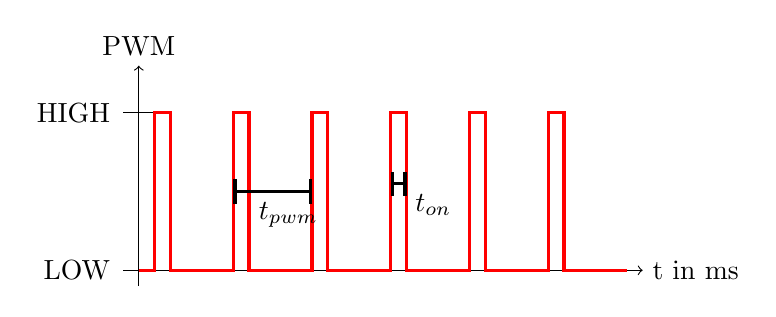
\begin{tikzpicture}
    \draw[->] (-0.4,0) -- (6.2,0) node[right] {t in ms};
    \draw[->] (-0.2,-0.2) -- (-0.2,2.6) node[above] {PWM};   
    \draw[] (-.4,2) -- (0,2) node[pos=-0.1, left] {HIGH};
    \draw[] (-.4,0) -- (0,0) node[pos=-0.1, left] {LOW};
     
    \draw[color=red,very thick] plot coordinates {(-0.2,0) (0,0) (0,2)(.2,2) (.2,0) (1,0) (1,2) (1.2,2) (1.2,0) (2,0) (2,2) (2.2,2)(2.2,0) (3,0) (3,2) (3.2,2)(3.2,0) (4,0) (4,2) (4.2,2)(4.2,0) (5,0) (5,2) (5.2,2)(5.2,0) (6,0)};
    
    \draw[|-|,very thick] (1,1) -- (2,1 )
        node[pos=0.7,below]{$t_{pwm}$}; 
    \draw[|-|,very thick] (3,1.1) -- (3.2,1.1 )
        node[pos=2.7,below]{$t_{on}$};     
  \end{tikzpicture}
}

\subfigure[Mittelstellung und maximale Drehung nach links und rechts]{\includegraphics[width=0.9\textwidth]{Kapitel3/Tikz/servoPWM}}

\caption{Der Zusammenhang zwischen Pluslänge des PWM Signals und Drehwinkel des Servus}
\label{fig:pwm}
\end{center}
\end{figure}

Die Zeiten `t periode'' und ``t on'' bestimmen den Servowinkel. In der  Tabelle 
\ref{tab:servopwmtime} stehen die Parameter die von einem Standard-Servo verarbeitet werden. 
Mit diesen Parametern ist ein Servo aber noch nicht vollständig ausgesteuert. Generiert man 
die Signale selber kann man noch mehr Drehwinkel aus dem Servo herausholen. Die maximalen 
Werte müssen für jeden Servotyp experimentell bestimmt werden. Man tut dies, indem man ein 
PWM-Signal generiert das den Servo knapp an den mechanischen Endanschlag stossen lässt. 

\begin{table}[h]

\begin{center}

\tikzset{ 
    table/.style={
        matrix of nodes,
        row sep=-\pgflinewidth,
        column sep=-\pgflinewidth,
        nodes={
            rectangle,
            draw=black,
            align=center
        },
        minimum height=1.5em,
        text depth=0.5ex,
        text height=2ex,
        nodes in empty cells,
%%
        every even row/.style={
            nodes={fill=gray!20}
        },
        column 1/.style={
            nodes={text width=0.5\textwidth}
        },
        row 1/.style={
            nodes={
                fill=black!90,
                text=white,
                font=\bfseries
            }
        }
    }
}
\begin{tikzpicture}
\matrix (first) [table,text width=6em]
{
   Servo Type                             & t periode & t on min & t on max \\
   Standard-Servo                      & 20ms       & 1ms       & 2ms  \\
   Servo Futaba S3003             & 20ms & 0,58ms & 2,4ms \\
   Modellcraft VSD-5E-HS   (digital)    & 10ms &  0,5ms   & 2,3ms \\
};
 \end{tikzpicture}
\end{center}
\caption{Parameter für verschiedene Servos }
\label{tab:servopwmtime}
\end{table}%


\subsection{Aufbau der Schaltung}

Gab es früher je nach Herstellerfirma unterschiedliche Stecksysteme, so hat sich im Laufe der Zeit der
 sog. Uni-Anschluss durchgesetzt. Elektrisch ist der Uni-Stecker so aufgebaut, dass er das in der 
 Elektronik übliche 2.54mm Rastermaß benutzt. Er passt also problemlos auf unser Breadboard.

Dieser Stecker ist mit einem 3-poligen Flachband-Kabel mit der eigentlichen Servoelektronik verbunden.
Gebräuchlich sind einige verschiedene Farbschemen bei diesen Kabeln:

\begin{itemize}
\item schwarz - rot - weiß
\item schwarz - rot - gelb
\item braun - rot - orange
\item schwarz - rot - blau
\end{itemize}

Das schwarz Kabel ist meistens GND und das rot Kabel  die Spannungsversorgung (5Volt). Die dritte Leitung (weiß, gelb, orange, blau, ...) ist die Signalleitung, über die das Servo mit Pulsen versorgt wird, welche ihm die anzufahrende Position mitteilen. Wenigstens in einem Punkt sind sich aber alle Hersteller einig: Die Versorgungsspannung wird immer über die mittlere der 3 Adern des Flachbandkabels geführt, die auch immer rot ausgeführt wird.
\marginfigure{Kapitel3/Bilder/ServoSchaltung_breadboard}{Servomotor}{fig:ServoSchaltung_breadboard}


\subsection{Der Beispielsketch}

Mit dem folgenden Sketch (siehe Listing \ref{lst:servo_simple}) kann ein Servo betrieben werden ohne Hinzunahme von Bibliotheken. Dies kann von Vorteil sein, wenn man Platz auf dem Controller sparen möchte. Es ist hier darauf zu achten, das im folgenden Sketch der digitale Pin07 als Signal Pin für den Servo verwendet wird. Der Servo sollte in diesem Fall also auch entsprechend  angeschlossen sein.

Beim Ausführen des Sketchs bewegt sich der Servo einmal bis zum Anschlag (180 Grad) und dreht wieder zum entgegengesetzten Anschlag zurück. Das Ganze wiederholt sich anschließend.

In der Zeile \ref{lis:servo_postotime} wird die aktuelle Position von Grad in Millisekunden umgerechnet. Dabei entspricht ein Winkel von $0^\circ$ einer PWM-Plusweite von $200\text{ms}$.Ein Winkel von $180^\circ$ einer PWM-Pulsweite von $20\text{ms}$.

\begin{multicols}{2}
\begin{arduinoCode}{PWM Singnal wird erzeugt}{lst:servo_simple}
int servoPin = 3; /
int pwm;  (*@ \tikzmark{pwm} @*) 
int pos; 

void setup() {
   pinMode(servo, OUTPUT);
}

void loop() {
  for(pos=0; pos<180; pos++) {
    servoMove(servoPin, pos); (*@ \tikzmark{servoMove} @*) 
  }
}

void servoMove(int servo, int pos){
  // Winkel in Mikrosekunden umrechnen
  pwm = (pos * 11) + 200; (*@ \label{lis:servo_postotime} @*)  
  digitalWrite(servo, HIGH); (*@ \tikzmark{pwmHigh} @*)
  delayMicroseconds(pwm); // Dauer des PWM-Pluses
  digitalWrite(servo, LOW); // Servo Pin auf LOW Ende des PWM-Pluses
  delay(20); // 20 ms warten
}
\end{arduinoCode}
\columnbreak
\vfill\null 
\begin{itemize}
  \itemsep40pt
    \item[] \tikzmarkcomment{item1}{Mit dem Wert 0 bis 255 wird der Servowinkel gesteuert}
    \item[] \tikzmarkcomment{item2}{Die Funktion servoMove() berechnet aus der Winkelangabe (pos) die Dauer des PWM-Signal  in Millisekunden und erzeugt anschliessend das PWM-Signal. }
    \item[] \tikzmarkcomment{item3}{Servo Pin auf HIGH Beginn des PWM-Pluses}    
 \end{itemize}
\vfill \null

\begin{tikzpicture}[remember picture,overlay]
  \path[red, thick,-] (pwm.east) edge [out=0 , in=180] (item1);
  \path[red, thick,-] (servoMove.east) edge [out=0 , in=180] (item2);
  \path[red, thick,-] (pwmHigh.east) edge [out=0 , in=180] (item3);
\end{tikzpicture}
\end{multicols}

\subsection{Aufgaben}

\subsubsection{Aufgabe 1}
Baue die Schaltung in Abb. \ref{fig:ServoSchaltung_breadboard} nach und teste dann die zwei verschieden Arten (Listing \ref{lst:servo_simple} und \ref{lst:servo2}) einen Servo zu steuern. 
\subsubsection{Aufgabe 2}

Eine etwas einfachere Lösung zeigt Listing \ref{lst:servo2}. Hier wird auf die in der Arduino IDE
 enthaltene Servo Library zurückgegriffen.
 
\subsection{Die Servo Library} %TODO Servo Library fertig schreiben
 Das Beispiel findet sich auch in der IDE unter 
 File $->$ Examples $-> $ Servo.  Achtung: bei Listing \ref{lst:servo2} wird der digitale Pin09 verwendet.

\begin{arduinoCode}{Testsketch für die Servo-Library}{lst:servo2}
#include <Servo.h> 
 
Servo myservo;  // create servo object to control a servo 
                // a maximum of eight servo objects can be created 
 
int pos = 0;    // variable to store the servo position 
 
void setup() 
{ 
  myservo.attach(9);  // attaches the servo on pin 9 to the servo object 
} 
 
 
void loop() 
{ 
  for(pos = 0; pos < 180; pos += 1)  // goes from 0 degrees to 180 degrees 
  {                                  // in steps of 1 degree 
    myservo.write(pos);              // tell servo to go to position in variable 'pos' 
    delay(15);                       // waits 15ms for the servo to reach the position 
  } 
  for(pos = 180; pos>=1; pos-=1)     // goes from 180 degrees to 0 degrees 
  {                                
    myservo.write(pos);              // tell servo to go to position in variable 'pos' 
    delay(15);                       // waits 15ms for the servo to reach the position 
  } 
} 
\end{arduinoCode}

\subsection{Aufgaben}

\subsubsection{Aufgabe 1}


\subsubsection{Aufgabe 2}
Verändere beide Beispiel-Sketche so, dass sich der Servo um $90^\circ$ dreht. Verändere in Listing
\ref{lst:servo_simple} die Zeile \ref{lis:servo_postotime} entsprechend. 

\clearpage
\sectionInformatik{C Sprachstruktur: Library}
%TODO Sprachstruktur Library fertig schreiben

\clearpage
\section{DC-Motoren und externe Spannungsquelle}

DC-Motoren bestehen auf Dauermagneten und Spulen. In der Spule wird beim durchfließen des elektrischen Stromes ein Magnetfeld induziert (erzeugt). Dieses induzierte Magnetfeld und das Magnetfeld des Dauermagneten stoßen einander ab. Durch Schreifkontakte wird der Stromfluss durch die Spule an- bzw. aufgeschaltet. Dadurch entsteht  die Drehung des DC-Motors. Je stärker der Stromfluss ist, desto schneller dreht sich der DC-Motor. Ein normaler DC-Motor benötigt mehr als $100\mA$. Deshalb reicht die max. mögliche Strom der ein digitaler Port ($40mA$) nicht aus um einen DC-Motoren zu betreiben. Mit zwei Motoren kommt man auch schnell an die Grenzen des gesamten Arduino-Boards. Das Arduino-Board (Steuer-Stromkreis) wird deshalb nur als Schalter für einen Externen Stromkreis (Arbeit-Stromkreis) benutzt. Die Steuerung erfolgt mit Hilfe eines n-FET Transistors.   
\marginfigure{Kapitel3/Bilder/dcmotor-nfet}{DC-Motor mit externer Spannungsquelle}{fig:dcmotor-nfet}

\clearpage
\section{Integrierte Schaltkreise, IC}
Viele Schaltungen oder Schaltungsteile kommen in der praktischen Elektronik immer wieder vor. Um 
diese, teilweise komplexen, Schaltungen nicht immer wieder neu aufbauen oder erfinden zu müssen, 
werden sie in integrierte Schaltungen (IS = Integrierter Schaltkreis) zusammengefasst und in einem 
Gehäuse vergossen.

Integrierter Schaltungen sind preisgünstig, da als Massenprodukt gefertigt werden. Durch ihren
kompakten  Aufbau sind die zudem platzsparend und betriebssicher.
 
Vor der Entwicklung integrierter Schaltungen Ende der 1950er wurden elektrische Schaltungen mit 
diskreten Bauteilen aufgebaut, d. h. mit einzelnen Transistoren, Dioden, etc., welche auf einer 
Leiterplatte zu einer Schaltung zusammengefügt wurden. Dies war in Größe und Lebensdauer 
bereits ein wesentlicher Durchbruch gegenüber den damals konkurrierenden Elektronenröhren. 
Die Vorteile durch den Einsatz von Transistoren und Leiterplatten (Platinen), wie Verkleinerung 
und geringere Leistungsaufnahme, verdrängten die Systeme aus Elektronenröhren zunehmend. 
Dieser Trend verstärkte sich mit der Entwicklung und dem massiven Einsatz von integrierten 
Schaltungen ab den 1960ern.

Der erste integrierte Schaltkreis (ein Flipflop) wurde im September 1958 von Jack Kilby entwickelt.
Er bestand aus zwei Bipolartransistoren, welche auf einem Germanium-Substrat befestigt und durch 
Golddrähte verbunden wurden. Dieser Hybrid-Schaltkreis ist somit ein erstes Beispiel der Umsetzung 
der schon bekannten Transistor-Transistor-Logik (TTL) auf einen Schaltkreis. Sie war eine Vorstufe 
zur Weiterentwicklung der TTL-Schaltungen hin zu kleineren Bauformen. Schaltkreise aufgebaut aus 
solchen einfachen integrierten Schaltkreisen steuerten die Apollo Raumschiffe (siehe Abb.\ref{fig:ics3}).

Der erste „monolithische“, d. h. aus bzw. in einem einzigen einkristallinen Substrat gefertigt, 
integrierte Schaltkreis wurde von Robert Noyce im Juli 1959 zum Patent angemeldet. Das 
Entscheidende an Kilbys Erfindung war die komplette Fertigung der Bauelemente und 
Verdrahtung auf einem Substrat. Für die Herstellung wurden bereits fotolithografische 
Verfahren und Diffusionsprozesse genutzt. 

Die ersten integrierten Schaltkreise in Serienproduktion entstanden bereits Anfang der 1960er  
und bestanden lediglich aus bis zu wenigen Dutzend Transistoren (siehe Abb. \ref{fig:ics2}). Mit den Jahren wurden die
Bauelemente jedoch immer weiter verkleinert und auch passive Bauelemente wie Widerstände 
integriert sowie die Komplexität der integrierten Schaltkreise weiter erhöht. Damit erhöhte sich 
auch die Anzahl der Transistoren pro Chip beziehungsweise pro Chip-Fläche, dabei war die 
Anzahl der Transistoren die wichtigste Kenngröße von ICs.

\begin{figure}[htbp]
\begin{center}
\subfigure[IC in DIL/DIP \footnotemark]{\includegraphics[width=0.3\textwidth]{Kapitel3/Bilder/ic_three}}
\subfigure[TI SN5451, der erste kommerzielle IC \label{fig:ics2}]{\includegraphics[height=0.3\textwidth, angle=90]{Kapitel3/Bilder/KL_TI_SN5451_Logic_IC}}
\subfigure[Logisches NOR: IC aus dem PC, der das Apollo Raumschiff steuerte \label{fig:ics3}\footnotemark]{\includegraphics[width=0.28\textwidth]{Kapitel3/Bilder/Agc_nor2}}
\caption{IC im Gehäuse, der erste kommerzielle IC und der erste funktionsfähige IC}
\label{fig:ics}
\end{center}
\end{figure}
\addtocounter{footnote}{-1}\footnotetext{Dual In-Line (DIL), Gehäuse mit Anschlüssen an zwei Seiten, meist im Raster 2,54 mm (=100 mil), die „Urform“ der Chipgehäuse}
\addtocounter{footnote}{1}\footnotetext{Quelle: \url{http://www.ti.com/corp/docs/kilbyctr/downloadphotos.shtml}}

%\section{Shift Register und Ringzähler}
%
%\subsection{Shift Register}
%
%
%\subsection{Ringzähler}
%Der IC 4014 ist ein sogenannter Ringzähler. Er hat 10 Ausgänge. Bei jedem neuen Takt-Impuls am Clock-Eingang wird der nächste Ausgang auf HIGH gesetzt. 
%
%\marginfigure{Kapitel3/Bilder/shift-register}{Shift Register}{fig:shift-register}
%
%
%Die Beschaltung des ICs ist etwas verwirrend, aber man kann die Details ja im Datenblatt (erhältlich z.B. bei Conrad) nachlesen. Der Schalt-Impuls wird vom Arduino auf dem Digitalen Port 2 ausgegeben, indem dieser kurzzeitig auf HIGH und dann wieder auf LOW geschaltet wird. Der Arduino bezieht seinen Strom aus dem angeschlossenem USB-Kabel. Die Schaltung wird mit GND und 5V vom Arduino versorgt. An die Ausgänge des ICs werden 180 Ohm Widerstände und daran LEDs angeschlossen.
%
%\subsection{Der Arduino Sketch}
%
%
%
%
%\subsection{Aufgaben}
%
%\subsubsection{Aufgabe 1}
%Baue die Schaltung für das Shift-Register nach Abb. \ref{fig:shift-register} auf. 
%
%\subsubsection{Aufgabe 2}


\section{Der IC L293D zur Motorsteuerung}
\marginfigure{Kapitel3/Bilder/IC_L293D}{IC L293D}{fig:l293d}

\subsection{Die Brückenschaltung}

Wenn bei einem  DC-Motor die Laufrichtung umgekehrt werden soll, so muss die Richtung des 
elektrischen Stroms der den Motor durchfließt umgekehrt werden. Der einfachste Weg dies zu 
erreichen ist eine sogenannte H-Brückenschaltung. In der Abb. \ref{fig:brueckenschaltung} ist 
schematisch eine H-Brückenschaltung mit vier Schaltern dargestellt. 

\begin{figure}[h]
\begin{center}
\subfigure[Brückenschaltung]{ 
 \begin{circuitikz}
 
 \draw (1,-3) node[anchor=east]{GND} to[short, o-*] (2,-3) ;
 \draw (2,-3) to [-] (6,-3);
 
 \draw (2,-3) to[switch, l=$s_2$] (2,-1);
\draw (2,-1) to[switch, l=$s_1$] (2,1);

\draw (2,-1) to [R, l=$M$, *-*]   (6,-1);

 \draw (6,-3) to[switch, l=$s_4$] (6,-1);
\draw (6,-1) to[switch, l=$s_3$] (6,1);

 \draw (1,1) node[anchor=east]{$V_{dd}$} to[short, o-*] (2,1);
 \draw (2,1) to [-] (6,1);
 
\end{circuitikz}
}
\subfigure[vereinfachte Brückenschaltung mit FETs\label{fig:brueckenschaltung_d}]{ 
 \begin{circuitikz}
 
 \draw (1,-3) node[anchor=east]{GND} to[short, o-*] (2,-3) ;
 \draw (2,-3) to [-] (6,-3);
 
 \draw (2,-2) node[nmos](s2) {}
 	(s2.G)node[anchor=east] {pin02};
\path[-,thick]  (2,-3) edge  (s2.south east);
\draw (2,0) node[nmos](s1) {}
	(s1.G)node[anchor=east] {pin01};
\path[-,thick]  (s1.south east) edge  (s2.north east);
\path[-,thick]  (s1.north east) edge  (2,1);
\draw (2,-1) to [R, l=$M$, *-*]   (6,-1);


 \draw (6,-2) node[nmos](s4) {}
 	(s4.G)node[anchor=east] {pin04};
\path[-,thick]  (6,-3) edge  (s4.south east);	
\draw (6,0) node[nmos](s3) {}
	(s3.G)node[anchor=east] {pin03};
\path[-,thick]  (s3.south east) edge  (s4.north east);
\path[-,thick]  (s3.north east) edge  (6,1);

 \draw (1,1) node[anchor=east]{$V_{dd}$} to[short, o-*] (2,1);
 \draw (2,1) to [-] (6,1);
 
\end{circuitikz}
}
\subfigure[Moter dreht sich rechts herum]{ 
 \begin{circuitikz}
 
 \draw[color=red] (1,-3) node[anchor=east]{GND} to[short, o-*, i_<=$I$] (2,-3) ;
 \draw (2,-3) to [short] (6,-3);
 
 \draw[color=red] (2,-3) to [short, l=$s_2$, i_<=$I$,color=red]  (2,-1);
\draw (2,-1) to[switch, l=$s_1$] (2,1);

\draw[color=red] (2,-1) to [R, l=$M$,i<=$I$,*-*]   (6,-1);

 \draw (6,-3) to[switch, l=$s_4$] (6,-1);
\draw[color=red] (6,-1) to [short, l=$s_3$, i_<=$I$] (6,1);

 \draw[color=red] (1,1) node[anchor=east]{$V_{dd}$} to[short, o-*, i_>=$I$] (2,1);
 \draw[color=red] (2,1) to [short,  i_>=$I$] (6,1);
 
\end{circuitikz}
}
\subfigure[Moter dreht sich rechts herum]{ 
 \begin{circuitikz}
 
 \draw[color=red] (1,-3) node[anchor=east]{GND} to[short, o-*, i_<=$I$] (2,-3) ;
 \draw[color=red] (2,-3) to [short,  i_<=$I$] (6,-3);
 
 \draw(2,-3) to [switch, l=$s_2$] (2,-1);
\draw[color=red]  (2,-1) to [short, l=$s_1$, i_<=$I$,color=red]  (2,1);

\draw[color=red] (2,-1) to [R, l=$M$,i>=$I$,*-*]   (6,-1);

 \draw[color=red]  (6,-3) to [short, l=$s_4$, i_<=$I$]  (6,-1);
\draw (6,-1) to [switch, l=$s_3$] (6,1);

 \draw[color=red] (1,1) node[anchor=east]{$V_{dd}$} to[short, o-*, i_>=$I$] (2,1);
 \draw (2,1) to [short] (6,1);
 
\end{circuitikz}
}


  \caption{Brückenschaltung mit vier Schalter bzw. vier FET-Transistoren}
\label{fig:brueckenschaltung}
\end{center}
\end{figure}

\begin{table}[h]
\begin{center}
\tikzset{ 
    table/.style={
        matrix of nodes,
        row sep=-\pgflinewidth,
        column sep=-\pgflinewidth,
        nodes={
            rectangle,
            draw=black,
            align=center
        },
        minimum height=1.5em,
        text depth=0.5ex,
        text height=2ex,
        nodes in empty cells,
%%
        every even row/.style={
            nodes={fill=gray!20}
        },
        %column 1/.style={
          %  nodes={text width=2em,font=\bfseries}
        %},
        row 1/.style={
            nodes={
                fill=black!90,
                text=white,
                font=\bfseries
            }
        }
    }
}
\begin{tikzpicture}
\matrix (first) [table,text width=6em]
{
	$s_1$ & $s_2$ & $s_3$ & $s_4$ & Verhalten \\
	auf & auf & auf & auf & stop  \\
	auf & zu  & zu  & auf & links  \\
	zu  & auf & auf & zu  & rechts  \\
	zu  & zu  & auf & auf & Kurzschluss  \\
	auf & auf & zu  & zu  & Kurzschluss  \\
};
\end{tikzpicture}
\end{center}
\caption{Mögliche Schaltereinstellungen bei der Brückenschaltung }
\label{tab:brueckenschaltung}
\end{table}%
In der Tabelle \ref{tab:brueckenschaltung} sind die möglichen Schalterstellungen und das 
entsprechende Verhalten des Motors aufgelistet. Wenn nun diese vier Schalter durch 
FET-Transistoren ersetzt werden, ist den möglich mit Hilfe von vier digitalen Pins, die 
jeweils über einen Spannungsteiler mit dem Gate-Eingang der FETs verbunden werden 
eine H-Brückenschaltung zu realisieren, bei der mit Hilfe der digitalen Pins mit Motordrehrichtung 
gesteuert werden kann (vergleiche Abb. \ref{fig:brueckenschaltung_d}).     


\clearpage
\subsection{Pinbelegung des IC L293D}

Zum Glück müssen wir eine Brückenschaltung wie sie Abb. \ref{fig:brueckenschaltung_d}
ohne Spannungsteiler für jeden digitalen Pin zeigt nicht selber aufbauen. Diese Schaltung 
werden in ICs realisiert. Es gibt viele verschiedene Modelle und Marken von H-Bridge-ICs. 
Wir verwenden den IC L293D. Der L293D ist relative billig und ist ohne zusätzliche Kurzschluss-Dioden verwendbar. Deshalb ist er sehr einfach zu benutzen. In der Abb. \ref{fig:l293d1}
ist die Pinbelegung dargestellt. 

\marginfigure{Kapitel3/Bilder/L293D}{Pin Belegung}{fig:l293d1}
\marginfigure{Kapitel3/Bilder/IC_L293D}{IC L293D}{fig:l293d1-bauteil}
 
%\begin{figure}[h]
%\begin{center}
%\subfigure[Pin Belegung\label{fig:l293d1} ]{\includegraphics[width=0.45\textwidth]{Kapitel3/Bilder/L293D}}
%\subfigure[Bauteil]{\includegraphics[width=0.45\textwidth]{Kapitel3/Bilder/IC_L293D}}
%\caption{Die Pin Belegung und Aussehen des IC L293D}
%\label{fig:l293d}
%\end{center}
%\end{figure}


\begin{table}
\begin{center}
\tikzset{ 
    table/.style={
        matrix of nodes,
        row sep=-\pgflinewidth,
        column sep=-\pgflinewidth,
        nodes={
            rectangle,
            draw=black,
            align=center
        },
        minimum height=1.5em,
        text depth=0.5ex,
        text height=2ex,
        nodes in empty cells,
%%
        every even row/.style={
            nodes={fill=gray!20}
        },
        column 1/.style={
            nodes={text width=2.2em}
        },
       column 2/.style={
            nodes={text width=2.2em}
        },
       column 3/.style={
            nodes={text width=4em}
        },	
        column 6/.style={
            nodes={text width=0.4\textwidth}
        },
        row 1/.style={
            nodes={
                fill=black!90,
                text=white,
                font=\bfseries
            }
        },
        row 6/.style={
            nodes={text depth=3.5ex}
        }
  }
}
\begin{tikzpicture}
\matrix (first) [table,text width=6em]
{

``IN1'' & ``IN2''	& ``EN1'' & ``OUT1'' & ``OUT2'' & entspricht \\
0V &	 0V	&  5V &   - &  - & Motor kurzschließen (Bremsen)\\
0V &	 5V	& 5V	 &  -  & + & Motor dreht vorwärts\\
5V &	 0V	& 5V	 & +	& -  & Motor dreht rückwärts\\
5V &	 5V	& 5V	 & +  & + &Motor kurzschließen (Bremsen)\\
egal	& egal & 0V & hochohmig & hochohmig & Motor aus (Verbindung trennen, nicht kurzschließen)\\
};
\end{tikzpicture}
\end{center}
\caption{Übersicht der Pinbelegung für einen Motor (1,2) analog für Motor (3,4).}
\label{tab:brueckenschaltung}
\end{table}%

\clearpage
\subsection{Die Schaltung auf dem BreadBoard}
Das schwierige bei der Schaltung für den IC L293D ist, dass sie übersichtlich aufgebaut 
werden muss. In der Abb. \ref{fig:l293d} ist ein mögliche Aufbau dieser für zwei Motoren 
abgebildet. 

\marginfigure{Kapitel3/Bilder/L293D_breadboard}{L293D als Treiber für zwei DC-Motoren}{fig:l293d}


\subsection{Der Beispielsketch}
\begin{multicols}{2}
\begin{arduinoCode}{Testsketch für einen DC-Motor}{lst:dc-motor}
  const int motorPin1 = 5;  // IN1 (*@\tikzmark{inPin} @*)
  const int motorPin2 = 6;  // IN2
    
  void setup() {
    pinMode(motorPin1, OUTPUT); 
    pinMode(motorPin2, OUTPUT); 
  }

  void loop() {
    digitalWrite(motorPin1, HIGH); (*@\tikzmark{rueckwaerts} @*)
    digitalWrite(motorPin2, LOW);  
    delay(3000);
    
    digitalWrite(motorPin1, LOW);  (*@\tikzmark{stopp1} @*)
    digitalWrite(motorPin2, HIGH);
    delay(3000);
    
    digitalWrite(motorPin1, HIGH);  (*@\tikzmark{vorwaerts} @*)
    digitalWrite(motorPin2, LOW);  
    delay(3000);
    
    digitalWrite(motorPin1, LOW);  (*@\tikzmark{stopp2} @*)
    digitalWrite(motorPin2, LOW);
   }
\end{arduinoCode}

\columnbreak
\vfill\null 
\begin{itemize}
  \itemsep20pt
    \item[] \tikzmarkcomment{item1}{Die Motor PINs, wichtig ist, dass PWM-fähige PINs verwendet werden.}
    \item[] \tikzmarkcomment{item2}{Motor dreht sich rückwärts}
    \item[] \tikzmarkcomment{item3}{Motor stoppt}
    \item[] \tikzmarkcomment{item4}{Motor dreht sich vorwärts}
    \item[] \tikzmarkcomment{item5}{Motor stoppt}
 \end{itemize}
\vfill \null

\begin{tikzpicture}[remember picture,overlay]
  \path[red, thick,-] (inPin.east) edge [out=0 , in=180] (item1);
  \path[red, thick,-] (rueckwaerts.east) edge [out=0 , in=180] (item2);
  \path[red, thick,-] (stopp1.east) edge [out=0 , in=180] (item3);
  \path[red, thick,-] (vorwaerts.east) edge [out=0 , in=180] (item4);
  \path[red, thick,-] (stopp2.east) edge [out=0 , in=180] (item5);
\end{tikzpicture}
\end{multicols}

\subsection{Aufgaben}
Bau die Schaltung entsprechend Abb. \ref{fig:l293d} auf. Lade anschließend den Beispiel-Sketch \ref{lst:dc-motor} auf deinen Arduino.

\subsubsection{Aufgabe 1}
Verringere nun die Drehzahl deines Motors mit Hilfe eines PWM-Signals. Dazu musst du die digitalWrite-Befehle durch analogWrite ersetzen.
\margininfo{\textbf{Syntax:}\\
analogWrite(pin, value) \\
\textbf{Parameters:}\\
pin: the pin to write to.\\
value: the duty cycle: between 0 (always off) and 255 (always on). }

\subsubsection{Aufgabe 2}
Entwickle für die die drei verschiedene Zustände des Motor Routinen motorBackward, motorStop und motorForward. Übergabe Parameter sollen die PINs mit denen der Motor verbunden ist und ein PWM-Signal sein. 
\begin{arduinoCode}{}{}
void motorBackward(pin1,pin2,pwm) {
  // Code
}
\end{arduinoCode}

\subsubsection{Aufgabe 3 (Projekt)}
Im Beispiel-Sketch habe dich den Befehl delay() benutzt um den Motor eine definierte Zeit zu bewegen. Bau auf deinem Breadboard noch einen Push-Button hinzu und verwende die Methode aus Kapitel \ref{sec:millis}. Wenn der Push-Button gedrückt wird, soll der Motor stoppen. 


%\clearpage
%\section{Projekt: Deine eigene Motor Library}
%
%\subsection{Funktionsumfang der Library}
%
%\begin{multicols}{2}
%
%\begin{arduinoCode}{Testsketch für einen DC-Motor}{lst:motorlib1}
%
%// Use this code to test your motor with the Arduino board:
%
%// if you need PWM, just use the PWM outputs on the Arduino
%// and instead of digitalWrite, you should use the analogWrite command
%
%//  Motors
%int motor_left[] = {2, 3};
%int motor_right[] = {7, 8};
%
%//  Setup
%void setup() {
%  Serial.begin(9600);
%
%  // Setup motors
%  int i;
%  for(i = 0; i < 2; i++){
%    pinMode(motor_left[i], OUTPUT);
%    pinMode(motor_right[i], OUTPUT);
%  }
%}
%\end{arduinoCode}
%
%\begin{arduinoCode}{Testsketch für einen DC-Motor}{lst:motorlib2}
%//  Loop
%void loop() { 
%
%  drive_forward();
%  delay(1000);
%  motor_stop();
%  Serial.println("1");
%
%  drive_backward();
%  delay(1000);
%  motor_stop();
%  Serial.println("2");
%
%  turn_left();
%  delay(1000);
%  motor_stop();
%  Serial.println("3");
%
%  turn_right();
%  delay(1000);
%  motor_stop();
%  Serial.println("4"); 
%
%  motor_stop();
%  delay(1000);
%  motor_stop();
%  Serial.println("5");
%}
%
%\end{arduinoCode}
%
%
%\begin{arduinoCode}{Testsketch für einen DC-Motor}{lst:motorlib3}
%//  Drive
%
%void motor_stop(){
%  digitalWrite(motor_left[0], LOW); 
%  digitalWrite(motor_left[1], LOW); 
%
%  digitalWrite(motor_right[0], LOW); 
%  digitalWrite(motor_right[1], LOW);
%  delay(25);
%}
%
%void drive_forward(){
%  digitalWrite(motor_left[0], HIGH); 
%  digitalWrite(motor_left[1], LOW); 
%
%  digitalWrite(motor_right[0], HIGH); 
%  digitalWrite(motor_right[1], LOW); 
%}
%
%void drive_backward(){
%  digitalWrite(motor_left[0], LOW); 
%  digitalWrite(motor_left[1], HIGH); 
%
%  digitalWrite(motor_right[0], LOW); 
%  digitalWrite(motor_right[1], HIGH); 
%}
%  
%void turn_left(){
%  digitalWrite(motor_left[0], LOW); 
%  digitalWrite(motor_left[1], HIGH); 
%
%  digitalWrite(motor_right[0], HIGH); 
%  digitalWrite(motor_right[1], LOW);
%}
%
%void turn_right(){
%  digitalWrite(motor_left[0], HIGH); 
%  digitalWrite(motor_left[1], LOW); 
%
%  digitalWrite(motor_right[0], LOW); 
%  digitalWrite(motor_right[1], HIGH); 
%}
%\end{arduinoCode}
%\end{multicols}
%\clearpage

%%%%%%%%%%%%%%%%%%%%%%%%%%%%%%%%%%%%%
%%% Schrittmotoren %%%%%%%%%%%%%%%%%%
%%%%%%%%%%%%%%%%%%%%%%%%%%%%%%%%%%%%%
\section{Schrittmotoren} 
%TODO Schrittmotoren Schaltbild und Schaltung 


Bisher haben wir sog. Gleichstrom-Motoren verwendet. Wird  ein Gleichstrom-Motor mit einer passenden Betriebsspannung versorgt, so fängt er sich sofort an zu drehen. Die Drehzahl hängt dabei von der Leistung der Spannungsversorgung ab. Wenn ein Batterie zum Betrieb verwendet wird dreht sich der Motor langsamer, wenn die Batterie langsam leer wird. Bei spielen Einsatzbereichen ist aber eine genaue Kontrolle der Bewegung nötig.     


Um einen Schrittmotor zu steuern benötigst du ebenfalls  ein Treiber-Chip. Hier kann auch der L293D verwendet werden.

\subsection{Funktionsweise eines Schrittmotors}


\subsubsection{Beispiel-Sketch}
\begin{multicols}{2}
\null\vfill 
\begin{arduinoCode}{Testsketch für einen DC-Motor}{lst:dc-motor}

#include <Stepper.h> (*@\tikzmark{stepperLib}@*)
 
#define STEPS 100 (*@\tikzmark{steps}@*)
 
Stepper stepper(STEPS, 8, 9, 10, 11); (*@\tikzmark{stepperPins}@*)
 
int previous = 0;
 
void setup(){
  stepper.setSpeed(30);  (*@\tikzmark{speed}@*)
}
 
void loop(){
  int val = analogRead(0); (*@\tikzmark{sensor}@*)
  stepper.step(val - previous); (*@\tikzmark{move}@*)
  previous = val;
}
\end{arduinoCode}
  \vfill\null 
  \columnbreak
  \vfill\null 
  \begin{itemize}
    \itemsep15pt
    \item[] \tikzmarkcomment{item1}{Die Stepper Bibliothek wird eingebunden}
    \item[] \tikzmarkcomment{item2}{Anzahl der Schritte pro Umdrehung wird definiert}
    \itemsep25pt
    \item[] \tikzmarkcomment{item3}{Ein Objekt  Stepper wird erzeugt und mit den PINs verbunden}
    \item[] \tikzmarkcomment{item4}{Setzt die Rotationsgeschwindigkeit auf Umdrehungen pro Minute}
    \item[] \tikzmarkcomment{item5}{Sensorwert zur Drehung des Motor wird gemessen (Potentiometer)}
    \item[] \tikzmarkcomment{item6}{Der Stepper wird je nach Messwertwert gedreht.}
 \end{itemize}
\vfill \null

\begin{tikzpicture}[remember picture,overlay]
  \path[red, thick,-] (stepperLib.east) edge [out=0 , in=180] (item1);
  \path[red, thick,-] (steps.east) edge [out=0 , in=180] (item2);
  \path[red, thick,-] (stepperPins.east) edge [out=0 , in=180] (item3);
  \path[red, thick,-] (speed.east) edge [out=0 , in=180] (item4);
  
  \path[red, thick,-] (sensor.east) edge [out=0 , in=180] (item5);
  \path[red, thick,-] (move.east) edge [out=0 , in=180] (item6);
\end{tikzpicture}
\end{multicols}


\subsection{Schrittmotor mit dem Motortreiber A4988}

Wesentlich Komfortabler geht es mit Hilfe des Schrittmotor Treibers A4988 und der zugehörigen Library.  





\marginfigure{Kapitel3/Bilder/nema17A4988.png}{nema 17}{fig:nema17A4988}



%%%%%%%%%%%%%%%%%%%%%%%%%%%%%%%%%%%%%
%%% LCD-Displays %%%%%%%%%%%%%%%%%%%%
%%%%%%%%%%%%%%%%%%%%%%%%%%%%%%%%%%%%%
\section{Display}
%TODO Besser digitales Display  


\marginfigure{Kapitel3/Bilder/LCD.png}{LCD}{fig:lcd}


\subsection{Der Beispiel-Sketch}
\begin{multicols}{2}
\null \vfill
\begin{arduinoCode}{LCD-Display}{lst:lcd}
#include <LiquidCrystal.h> (*@\tikzmark{liqLib}@*)

LiquidCrystal lcd(12, 11, 5, 4, 3, 2); (*@\tikzmark{pins}@*)

void setup() {
  lcd.begin(16, 2); (*@\tikzmark{setCols}@*)
  // 
  lcd.print("hello, world!");(*@\tikzmark{hello}@*)
}

void loop() {
  lcd.setCursor(0, 1); (*@\tikzmark{setPos}@*)
  // :
  lcd.print(millis()/1000); (*@\tikzmark{printMes}@*)
}
\end{arduinoCode}
\vfill\null 
\columnbreak

\begin{itemize}
  \itemsep15pt
    \item[] \tikzmarkcomment{item1}{Die LiquidCrystal Bibliothek wird eingebunden}
    \item[] \tikzmarkcomment{item2}{PINs für das LCD-Displayplay}
    \item[] \tikzmarkcomment{item3}{Setup des LCD's  mit Anzahl der Spalten und Zeilen.}
    \itemsep20pt
    \item[] \tikzmarkcomment{item4}{Schreibt eine Nachricht auf das LCD.}
    \itemsep25pt
    \item[] \tikzmarkcomment{item5}{Setzt den Cursor auf die 0. Spalten in der 1. Zeile. (Beachte: Zeilen und Spalten werden von 0 an gezählt).}
    \itemsep35pt
    \item[] \tikzmarkcomment{item6}{Schreibt die Anzahl der Sekunden seit dem letzten 'reset' auf das Display.}
 \end{itemize}
\vfill \null

\begin{tikzpicture}[remember picture,overlay]
  \path[red, thick,-] (liqLib.east) edge [out=0 , in=180] (item1);
  \path[red, thick,-] (pins.east) edge [out=0 , in=180] (item2);
  \path[red, thick,-] (setCols.east) edge [out=0 , in=180] (item3);
  \path[red, thick,-] (hello.east) edge [out=0 , in=180] (item4);
  
  \path[red, thick,-] (setPos.east) edge [out=0 , in=180] (item5);
  \path[red, thick,-] (printMes.east) edge [out=0 , in=180] (item6);
\end{tikzpicture}
\end{multicols}


